\documentclass[12pt]{article}
\usepackage[english]{babel}
\usepackage[utf8]{inputenc} 
\usepackage[T1]{fontenc}
\usepackage{graphicx}
\usepackage{amsmath}
\usepackage{wrapfig}
\usepackage{enumerate}
\usepackage[top=1in, bottom=1.25in, left=1.1in, right=1.1in]{geometry}
\usepackage[dvipsnames]{xcolor}
\usepackage{subcaption}

\begin{document}

\begin{titlepage}

\newcommand{\HRule}{\rule{\linewidth}{0.5mm}} 

\center 

\textsc{\LARGE Universidad de Sonora}\\[1.5cm]
\textsc{\Large Licenciatura en Física}\\[0.5cm]
\textsc{\large Física Computacional I}\\[0.5cm]

\HRule \\[0.4cm]
{\huge \bfseries Evaluación 2}\\[0.4cm] 
\HRule \\[1.5cm]

\begin{minipage}{0.4\textwidth}
\begin{flushleft} \large
\emph{Alumno:}\\
José Gabriel Navarro I.
\end{flushleft}
\end{minipage}
~
\begin{minipage}{0.4\textwidth}
\begin{flushright} \large
\emph{Profesor:} \\
Carlos Lizarraga Celaya
\end{flushright}
\end{minipage}\\[2cm]

28 de Abril de 2018


\includegraphics[width=0.4\textwidth]{logo.png}\\
 
\vfill

\end{titlepage}

\section{Introducción}
En el presente reporte se habla acerca de la segunda evaluación de la materia Física Computacional I, que abarca el uso de Jupyter Lab, utilizando distintas librerías para la solución de un sistema de ecuaciones y sus posteriores graficas. En la presente evaluación, se resuelve el sistema atractor de Lorenz. \\

El atractor de Lorentz es un concepto que fue introducido por Edward Lorenz en 1963. Lorenz descubrió por primera vez el caos por accidente, cuando estaba realizando un modelo matemático para la convección atmosférica. Es por eso que este es un sistema dinámico determinista tridimensional no lineal derivado de las ecuaciones simplificadas de  convección que se producen en las ecuaciones dinámicas de la atmósfera terrestre. Las ecuaciones son: \\

\centerline{$ \dot x = a(y-x)$}
\centerline{$ \dot y = x(b-z) - y$}
\centerline{$ \dot z = xy - cz$}
$    $

Utilizando el codigo proporcionado por el blog de Geoff Boeing, se pudo hacer un análisis de este sistema para distintos parámetros de a, b y c, en nuestro caso: sigma, beta y rho. En donde se podrá observar las distintas graficas producidas y su interpretación correspondiente.

\section{Resultados}
Se utilizo el código proporcionado por Geoff Boeing para analizar el atractor de Lorentz utilizando Python, en donde se vio como hacer un gif y otro tipos de graficas. Se realizaron tres ejemplos distintos con distintos valores para sigma, beta y rho. A continuación se presentan los resultados obtenidos para distintos valores. \\

\subsection{Ejemplo 1}
Los valores para el primer ejemplo fueron los siguientes: \\

\centerline{$ sigma = 10$}
\centerline{$ beta = 8/3$}
\centerline{$ rho = 28$}
$    $

Las graficas obtenidas fueron la de fase en 3D, y para cada plano, además de la posición contra el tiempo. La fase en 3D es:

\pagebreak

\begin{figure}[h!]
    \centering
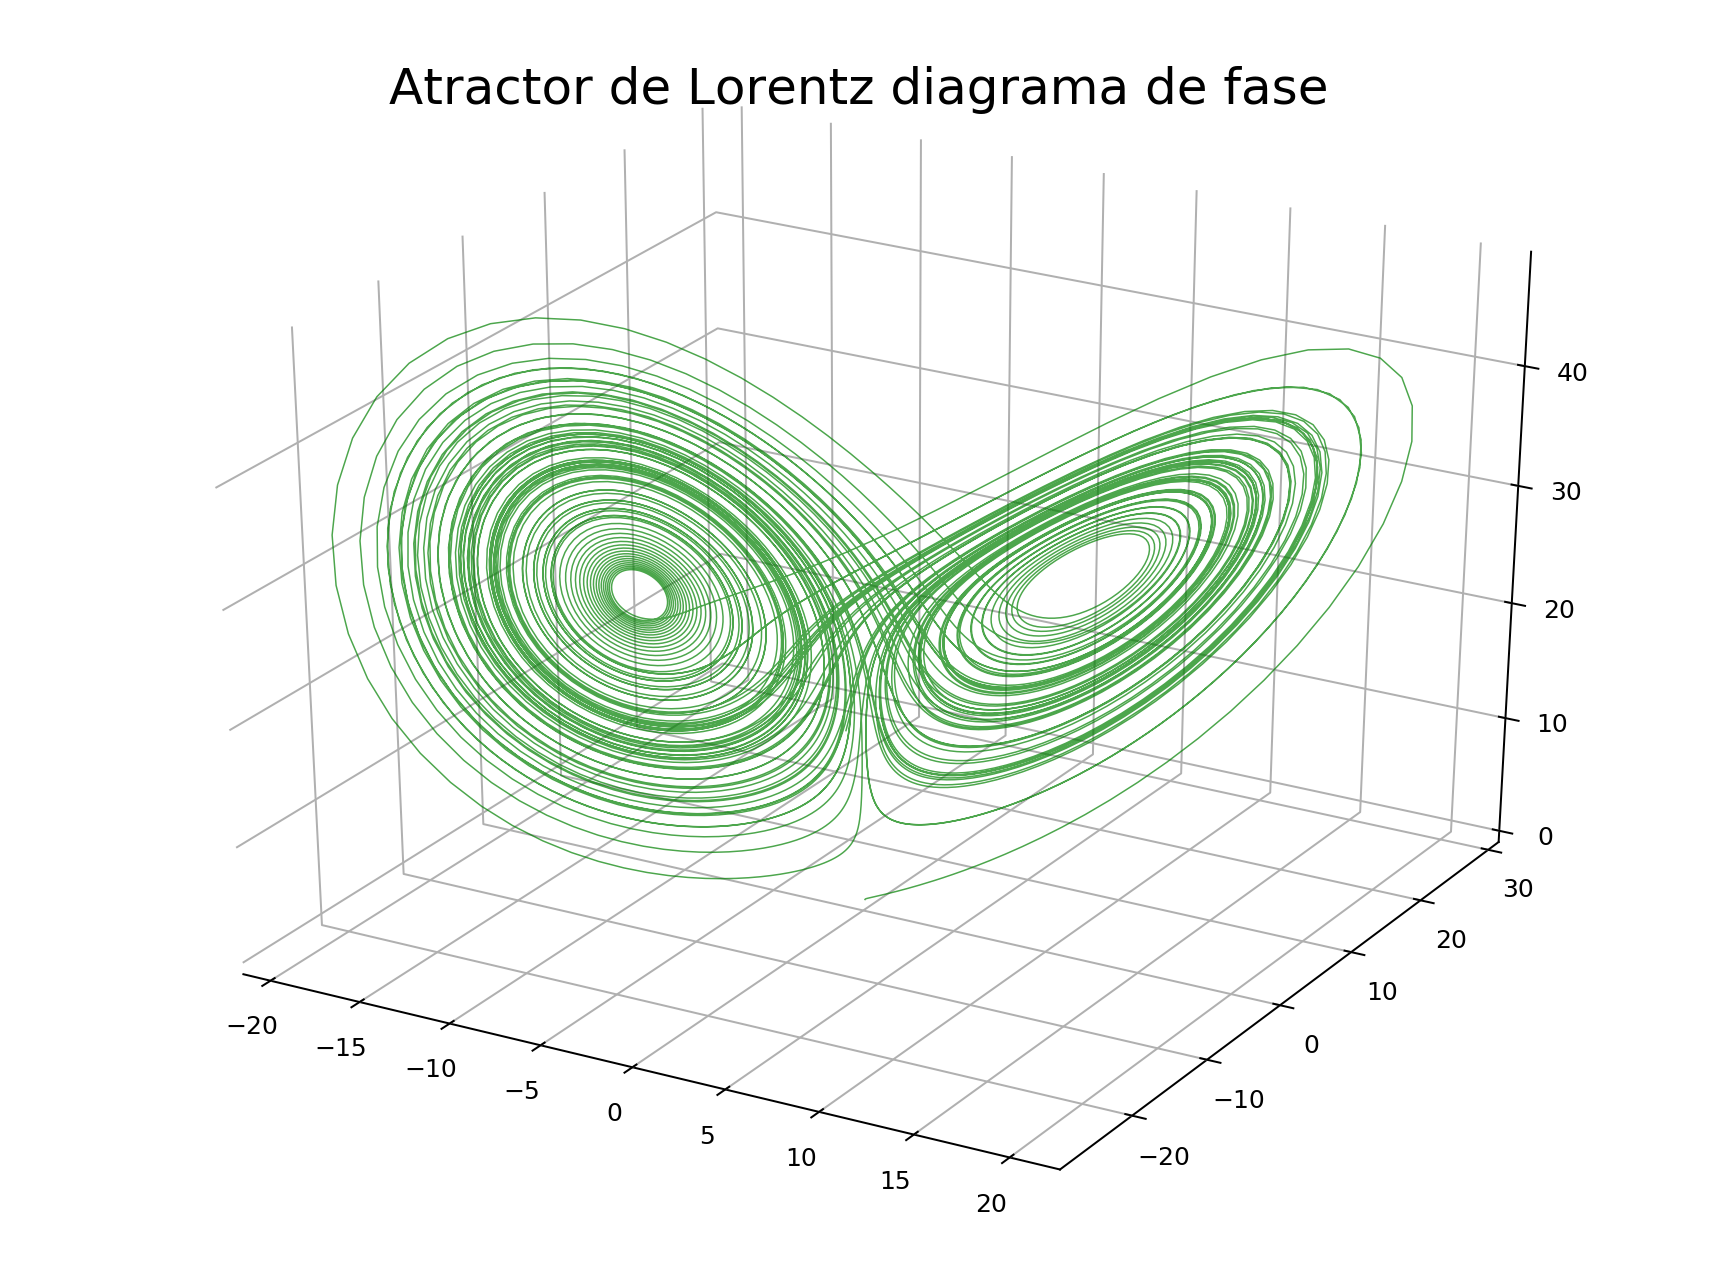
\includegraphics[width=5in]{AtractorLorentz3D1.png}
\end{figure}

En donde podemos observar como tiene una forma del número ocho pero doblado. Este modelo demuestra el caos atado a un ciertos valores para los parámetros y su atractor es fractal. Si analizamos el retrato de fase para cada plano obtenemos:

\begin{figure}[h!]
    \centering
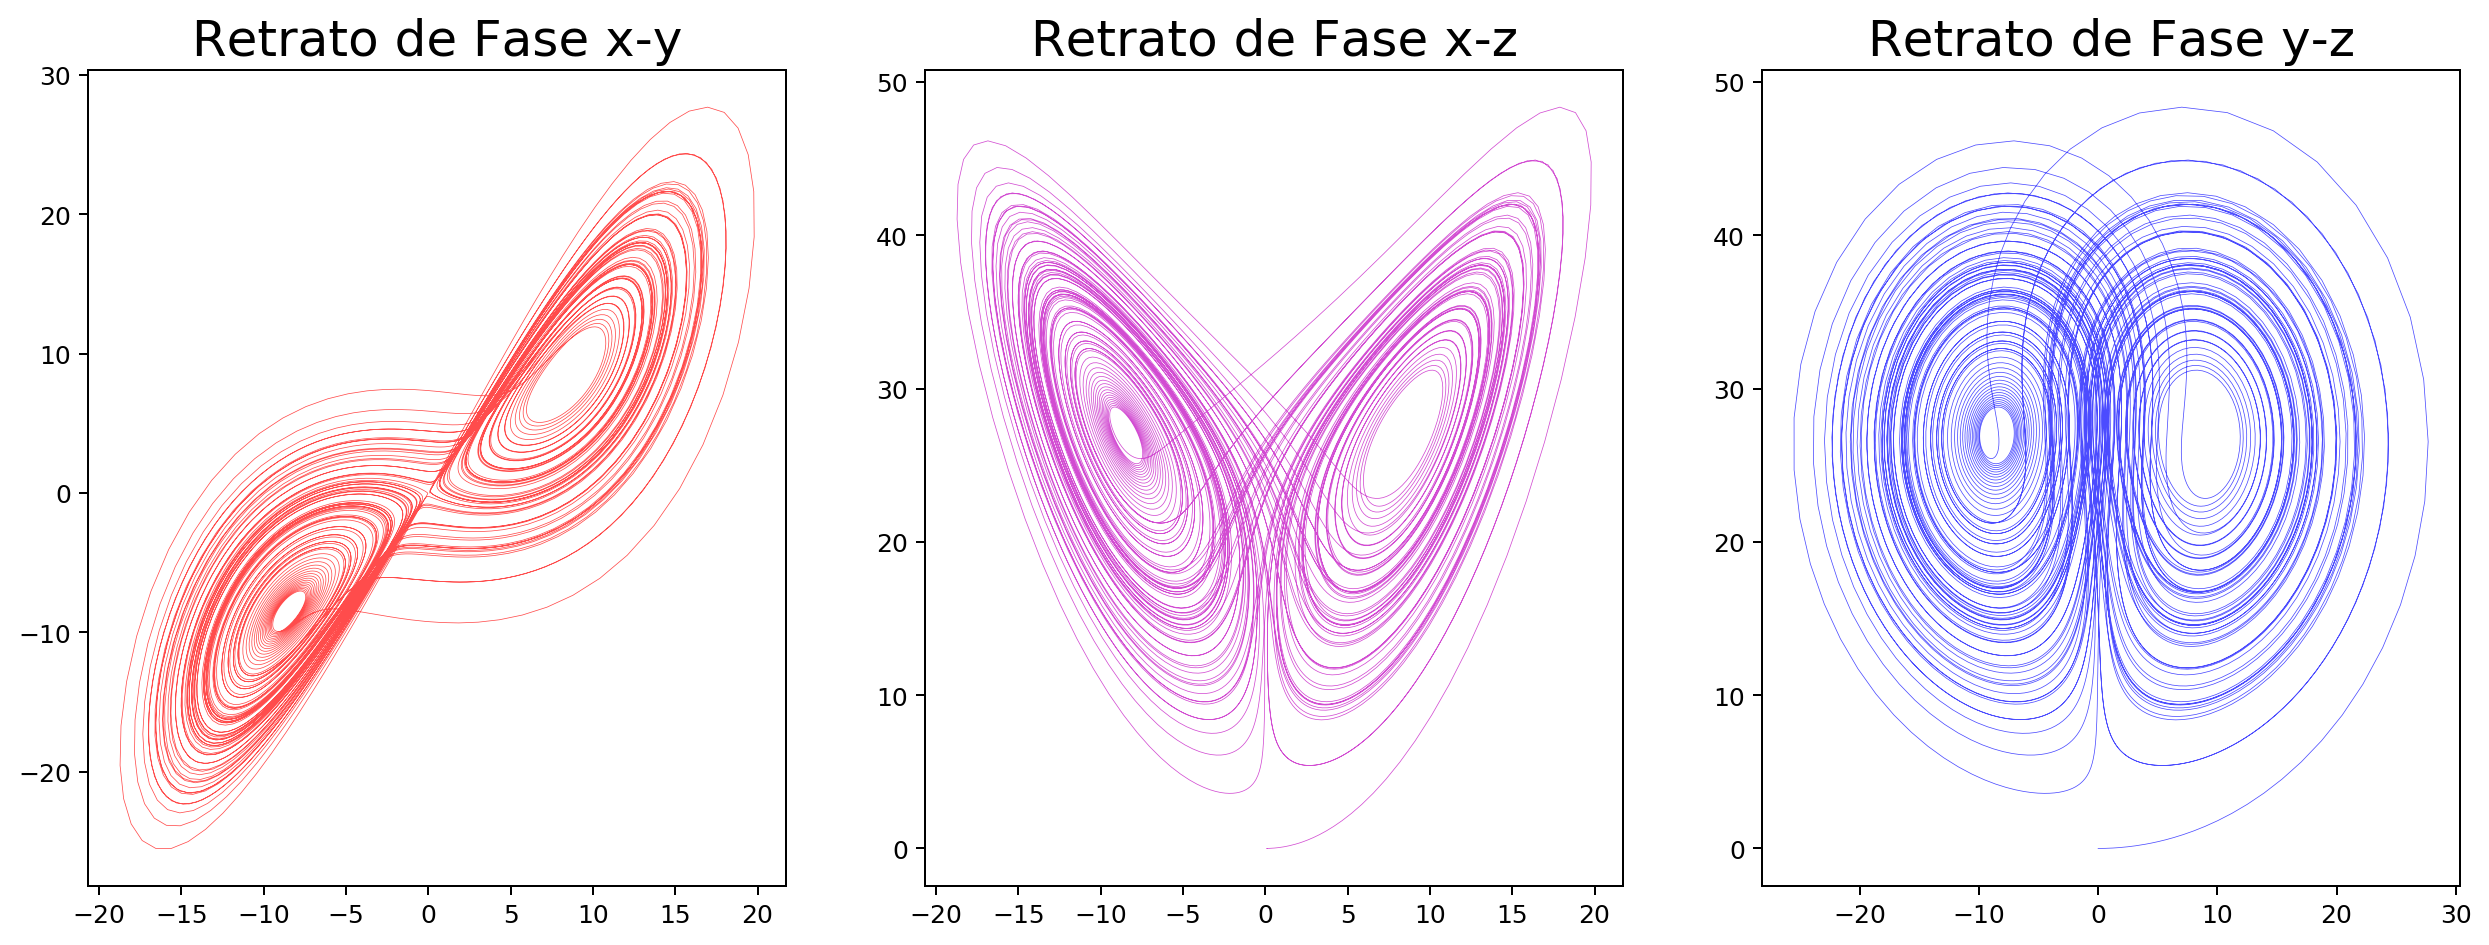
\includegraphics[width=5in]{AtractorLorentzFase1.png}
\end{figure}

Como podemos ver, para cada plano xy, xz, yz se tiene una distinta forma, donde en xy, se observa la figura de un ocho aplastado. Mientras que en x-z y y-z aparecen unas "mariposas".\\

La posición contra tiempo de cada una de las variables x, y, z resulto: 

\pagebreak

\begin{figure}[h!]
    \centering
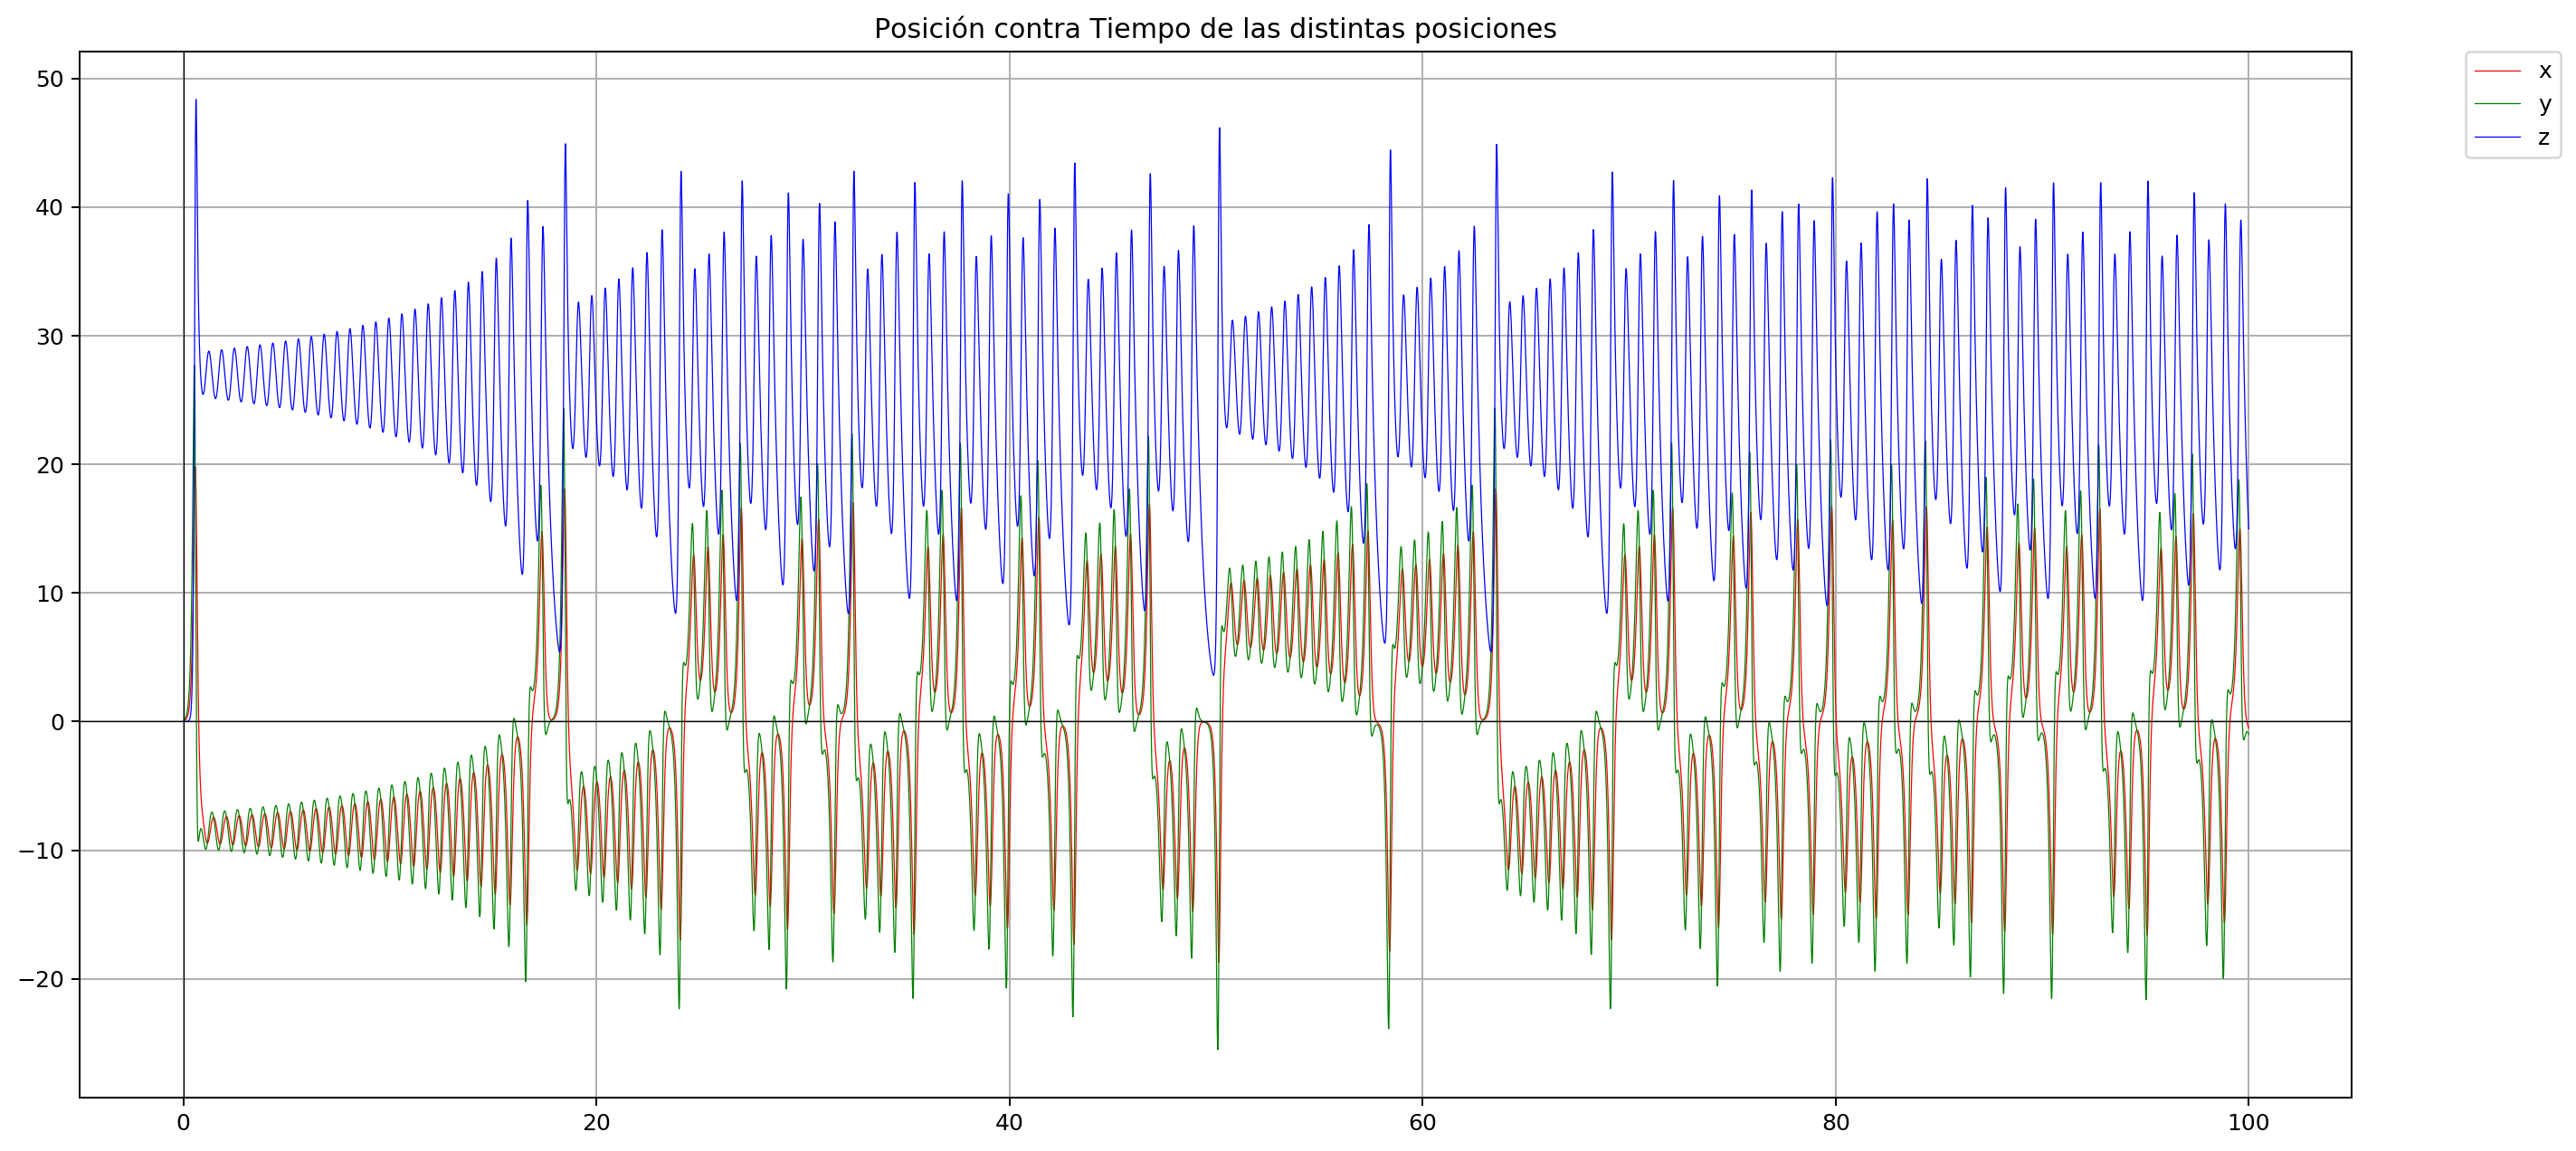
\includegraphics[width=5in]{AtractorLorentzPosicion1.png}
\end{figure}

Podemos observar como la posición en z oscila sobre cero, es decir, solo toma valores positivos, mientras que x y $y$ siguen mas o menos el mismo patrón y si pasan por la posición 0 en algún tiempo. Cabe mencionar que como el sistema es caótico, el sistema nunca pasará por una posición que ya haya atravesado. 

\subsection{Ejemplo 2}
Los valores para el segundo ejemplo fueron los siguientes: \\

\centerline{$ sigma = 28$}
\centerline{$ beta = 4$}
\centerline{$ rho = 46.92$}
$    $

El retrato de fase en 3D es el siguiente:

\begin{figure}[h!]
    \centering
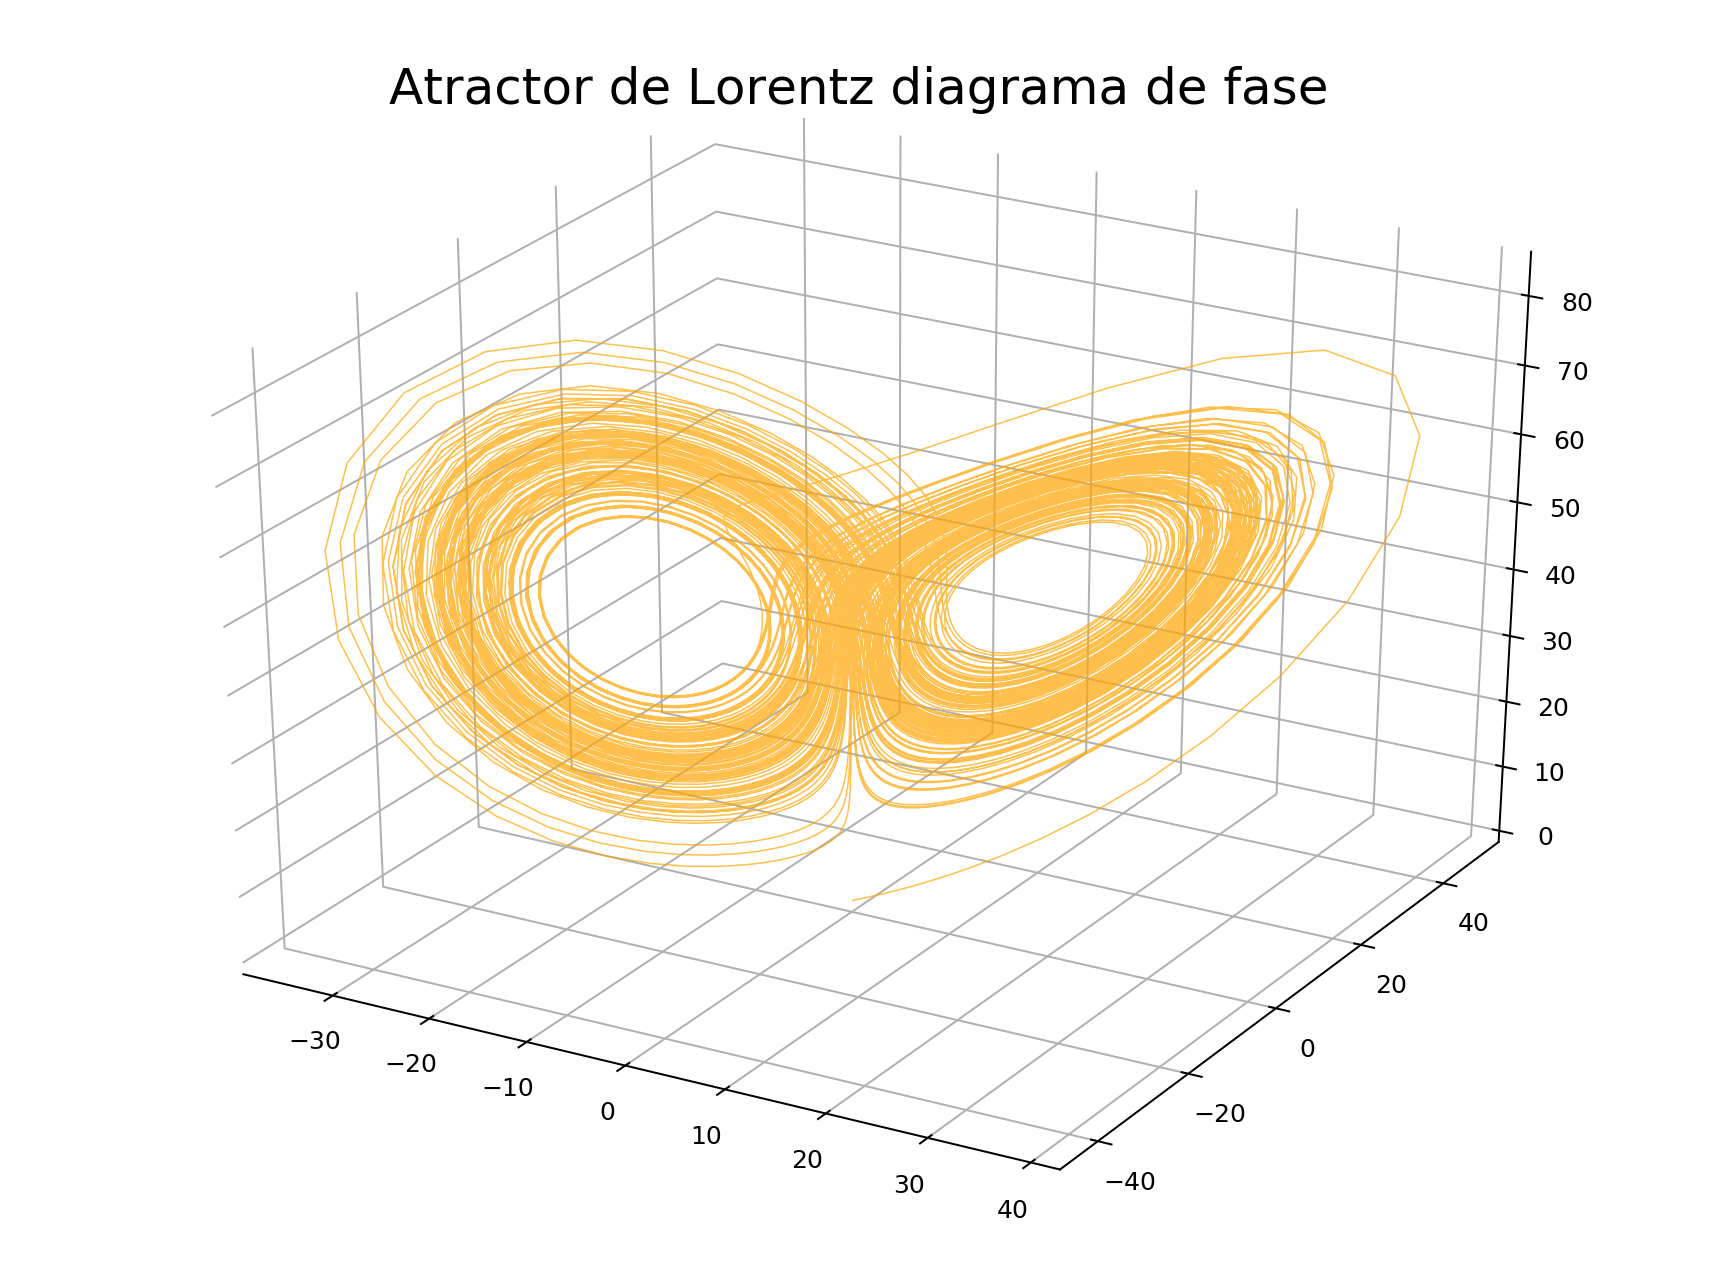
\includegraphics[width=4.5in]{AtractorLorentz3D2.png}
\end{figure}

Como se puede observar, la gráfica es muy parecida a la del primer ejemplo, pero esta vez la figura no se "rellena", ahora si tiene la forma de un ocho. Analizando el retrato de fase para cada plano:

\begin{figure}[h!]
    \centering
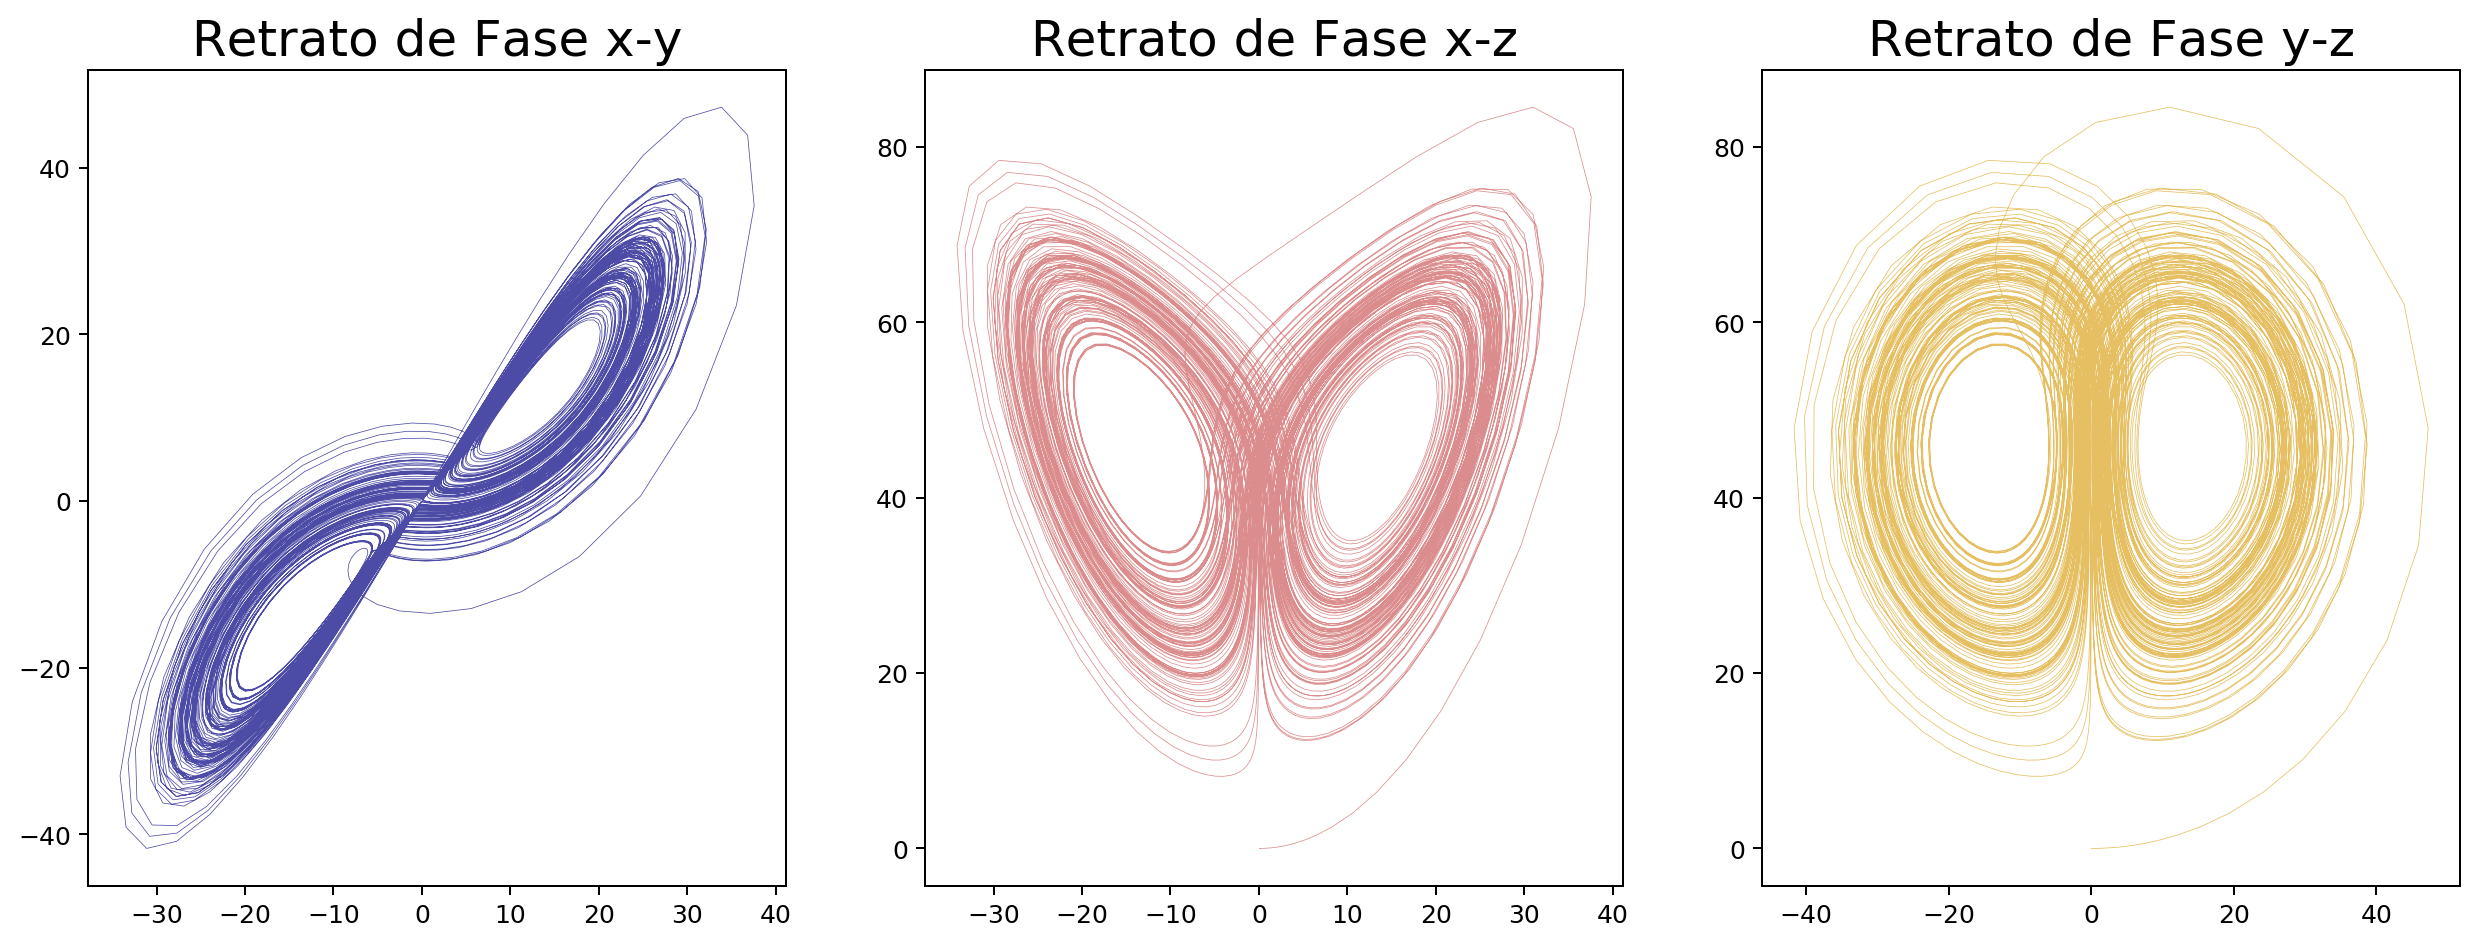
\includegraphics[width=5in]{AtractorLorentzFase2.png}
\end{figure}

De igual manera, son muy parecidas a las del primer ejemplo, pero tienen el "agujero" en el centro (al menos para el caso del plano x-y), mientras que x-z y y-z aparecen las mariposas. Por último, las posiciones contra el tiempo:

\begin{figure}[h!]
    \centering
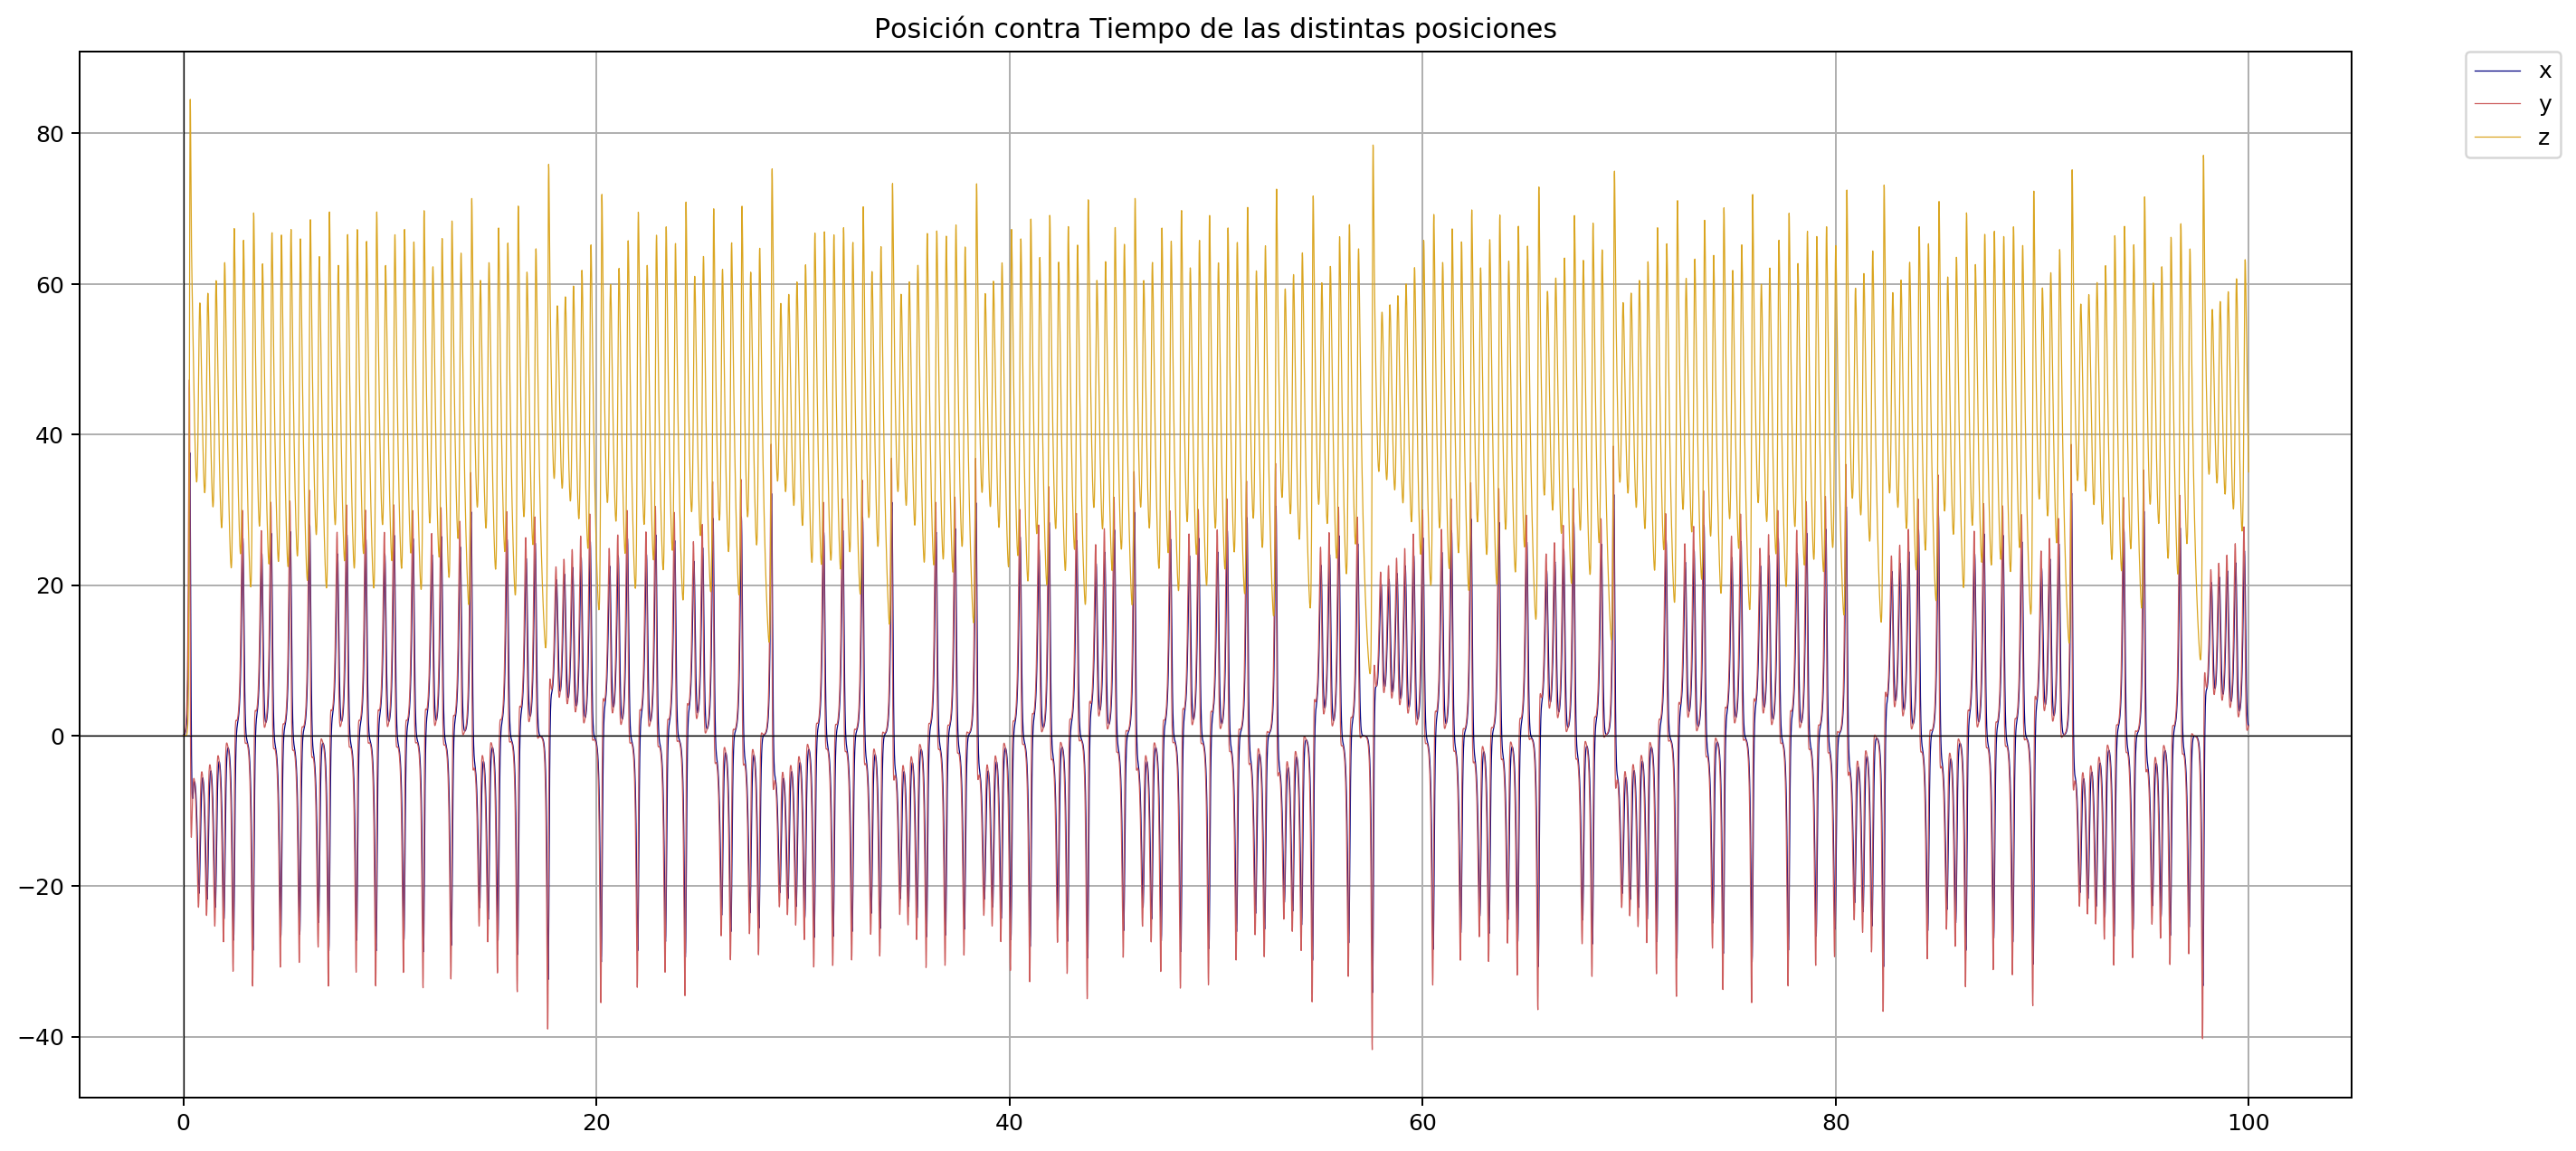
\includegraphics[width=5in]{AtractorLorentzPosicion2.png}
\end{figure}

Como se puede observar, existe una gran relación entre el ejemplo 1 y el ejemplo 2, ya que la posición en z es mayor a 0, y para x y $y$, pasa por 0, pero ahora presencia mas caos. 

\subsection{Ejemplo 3}
Los valores para el tercer ejemplo fueron los siguientes: \\

\centerline{$ sigma = 10$}
\centerline{$ beta = 8/3$}
\centerline{$ rho = 99.96$}
$    $

\pagebreak

El retrato de fase en 3D es:

\begin{figure}[h!]
    \centering
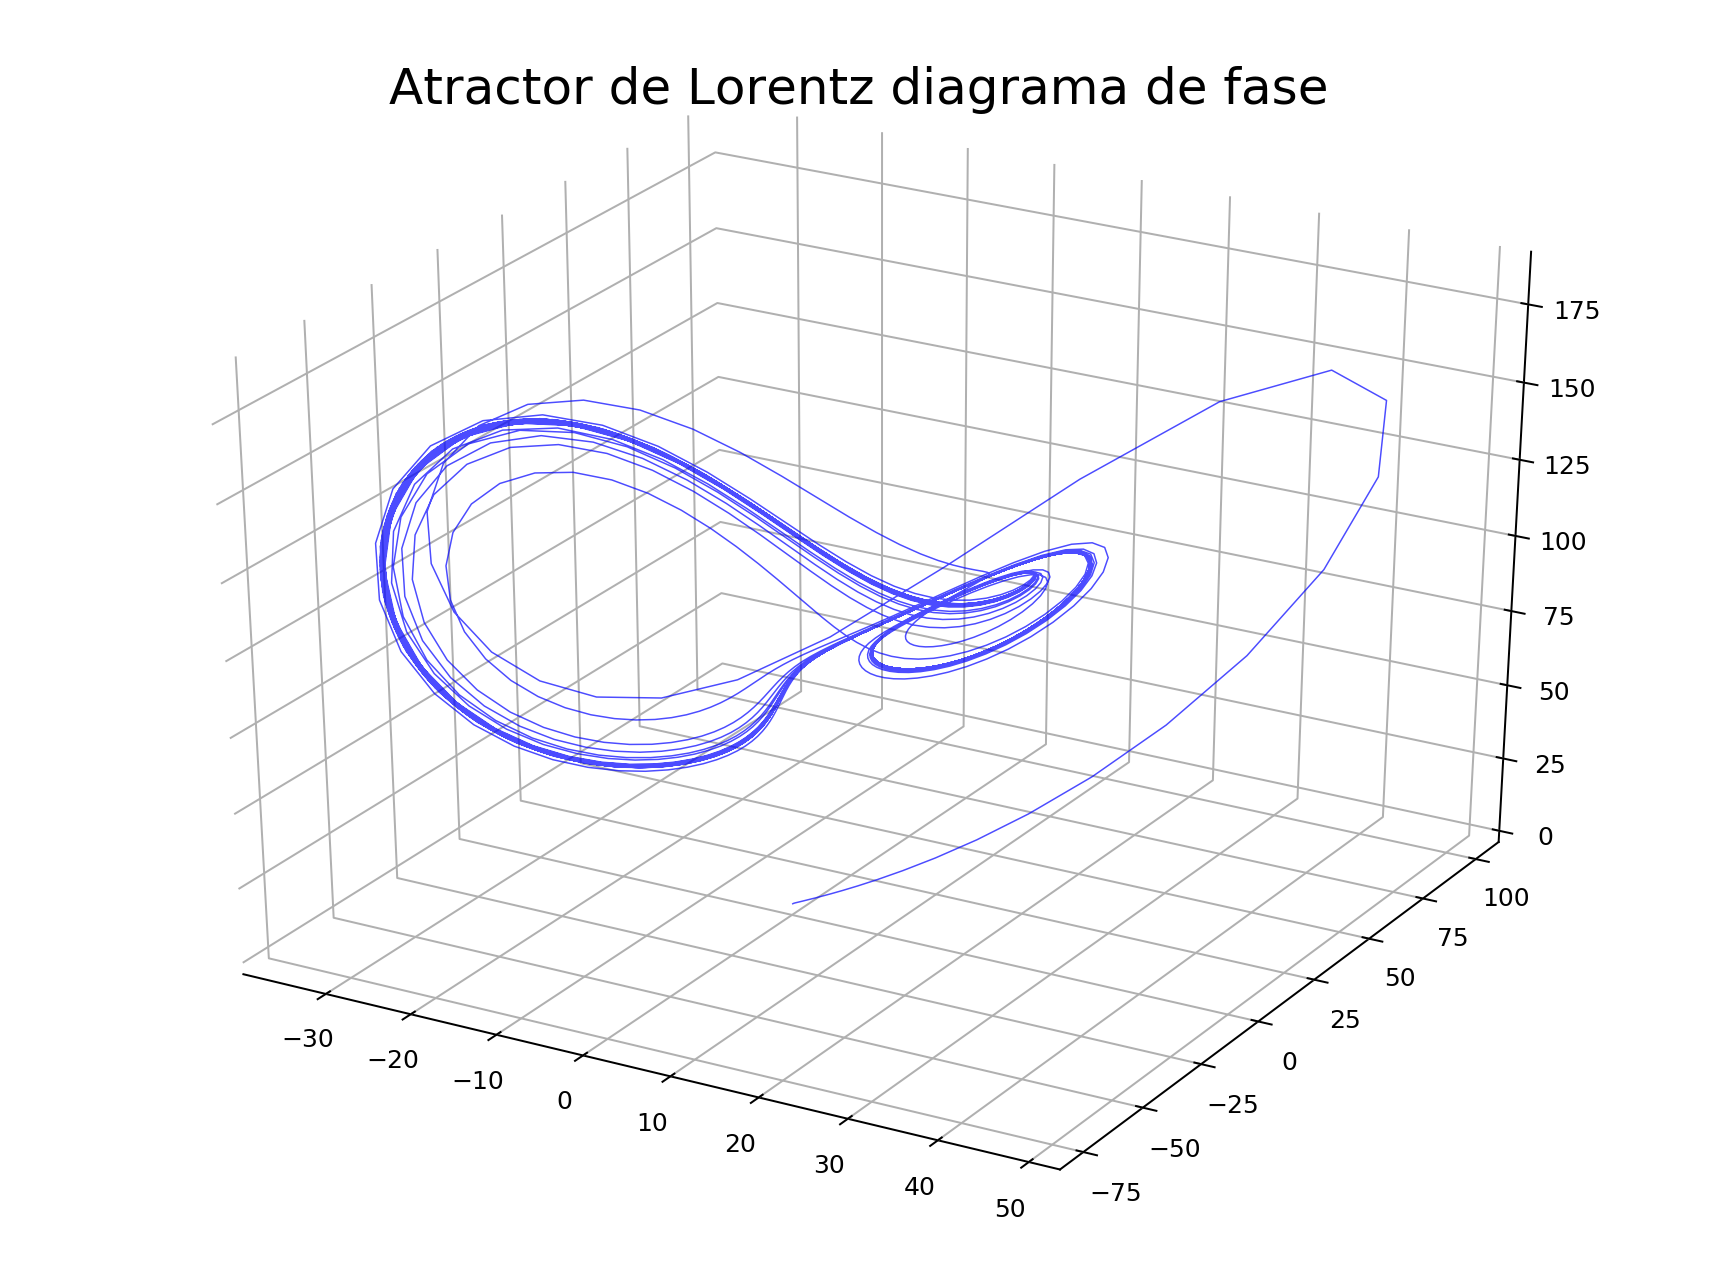
\includegraphics[width=5in]{AtractorLorentz3D3.png}
\end{figure}

Para este ejemplo ya no se sigue un patrón como los anteriores, si no que se mueve por distintos octantes con una cierta inclinación hacia el eje de las x negativo y valores mas altos para z. Los valores son iguales que en el ejemplo 1, excepto rho, así que de esto se puede concluir que hasta con un pequeño cambio en los parámetros, el sistema puede entrar a mas caos. Si observamos los retratos de fase para cada plano tenemos:

\begin{figure}[h!]
    \centering
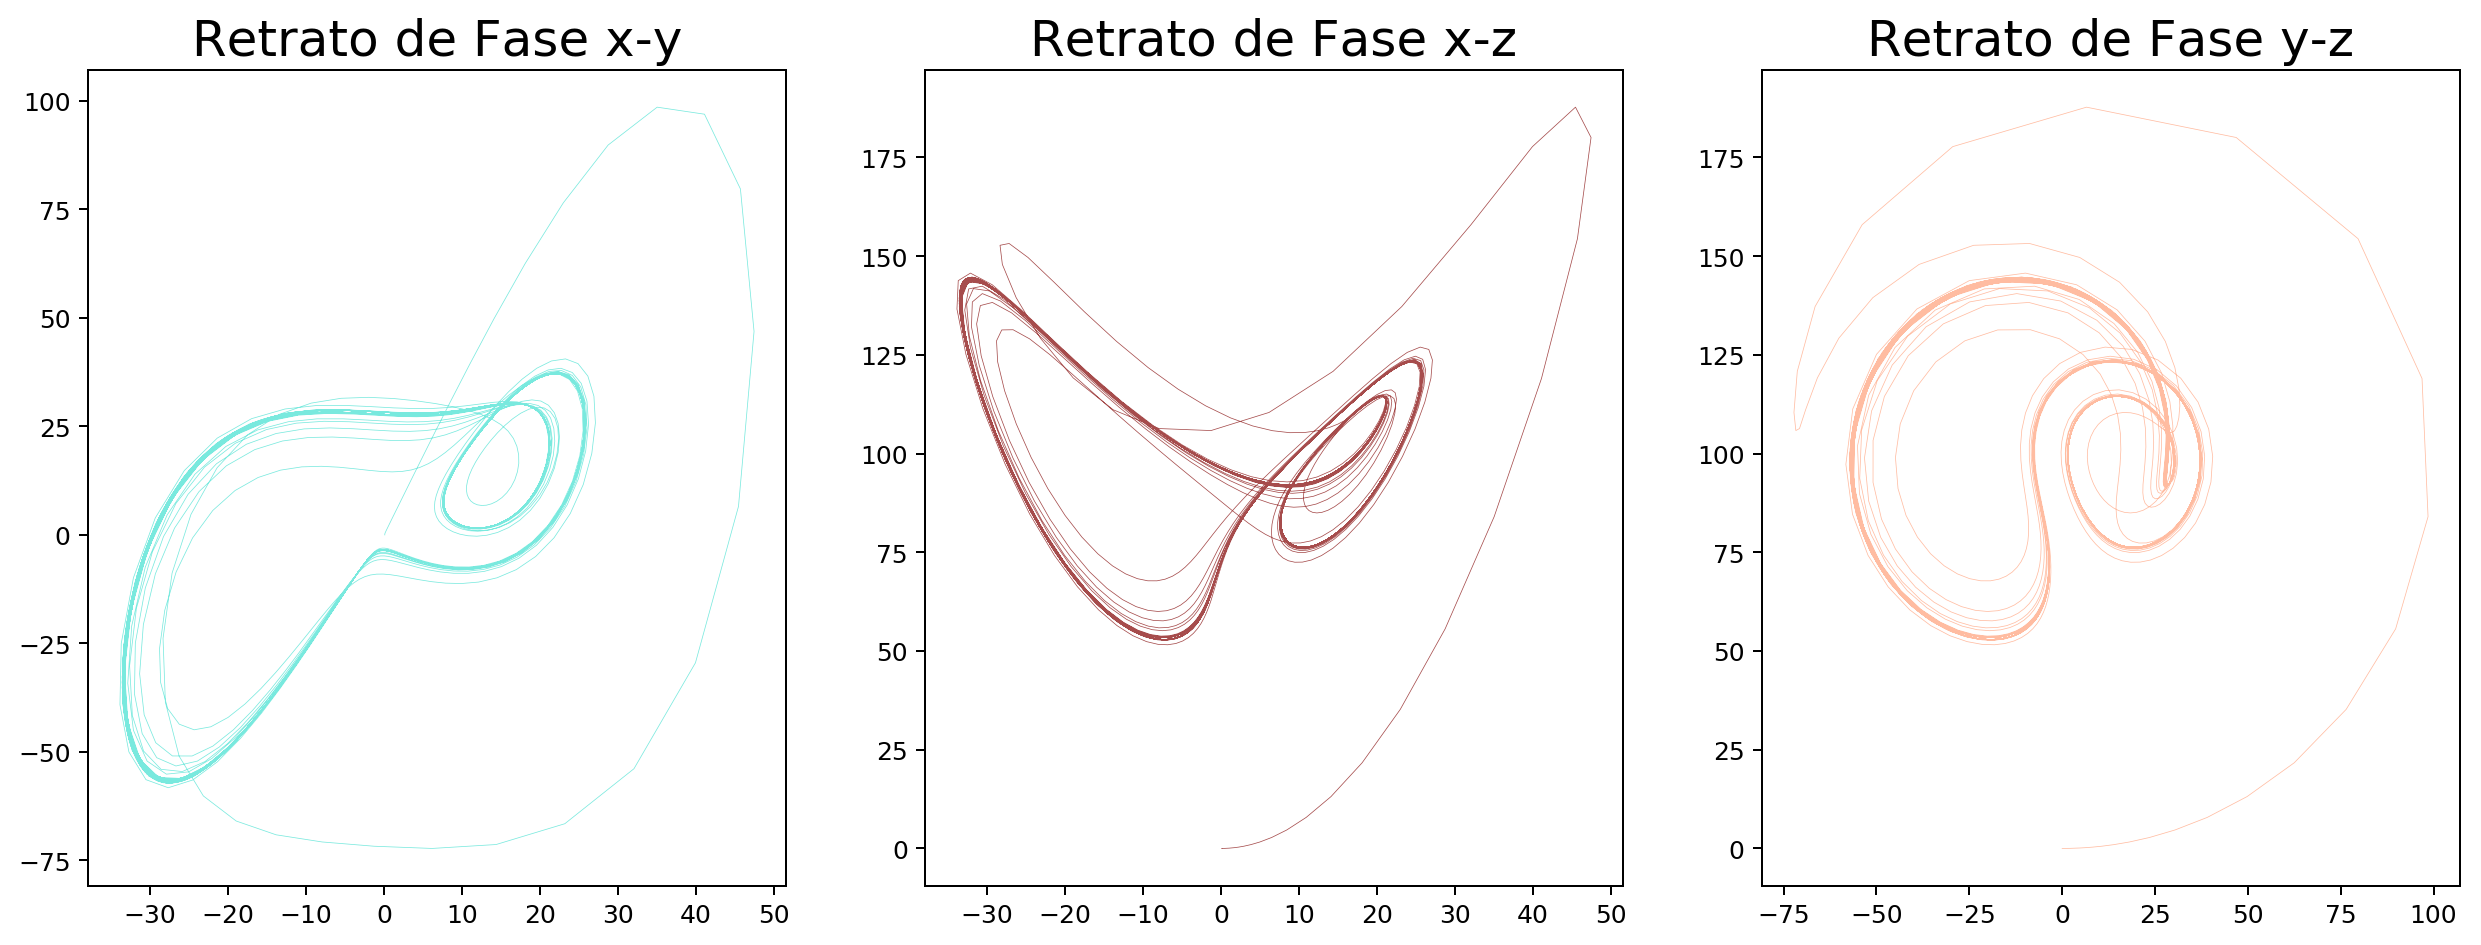
\includegraphics[width=5in]{AtractorLorentzFase3.png}
\end{figure}

A diferencia de los primeros dos ejemplos, se puede observar que este sistema es mas caótico, ya que no se puede observar ni la figura de un ocho, ni las mariposas, si no mas bien un patrón con forma circular u ovalada. Por último, analizando la posición contra tiempo:

\pagebreak

\begin{figure}[h!]
    \centering
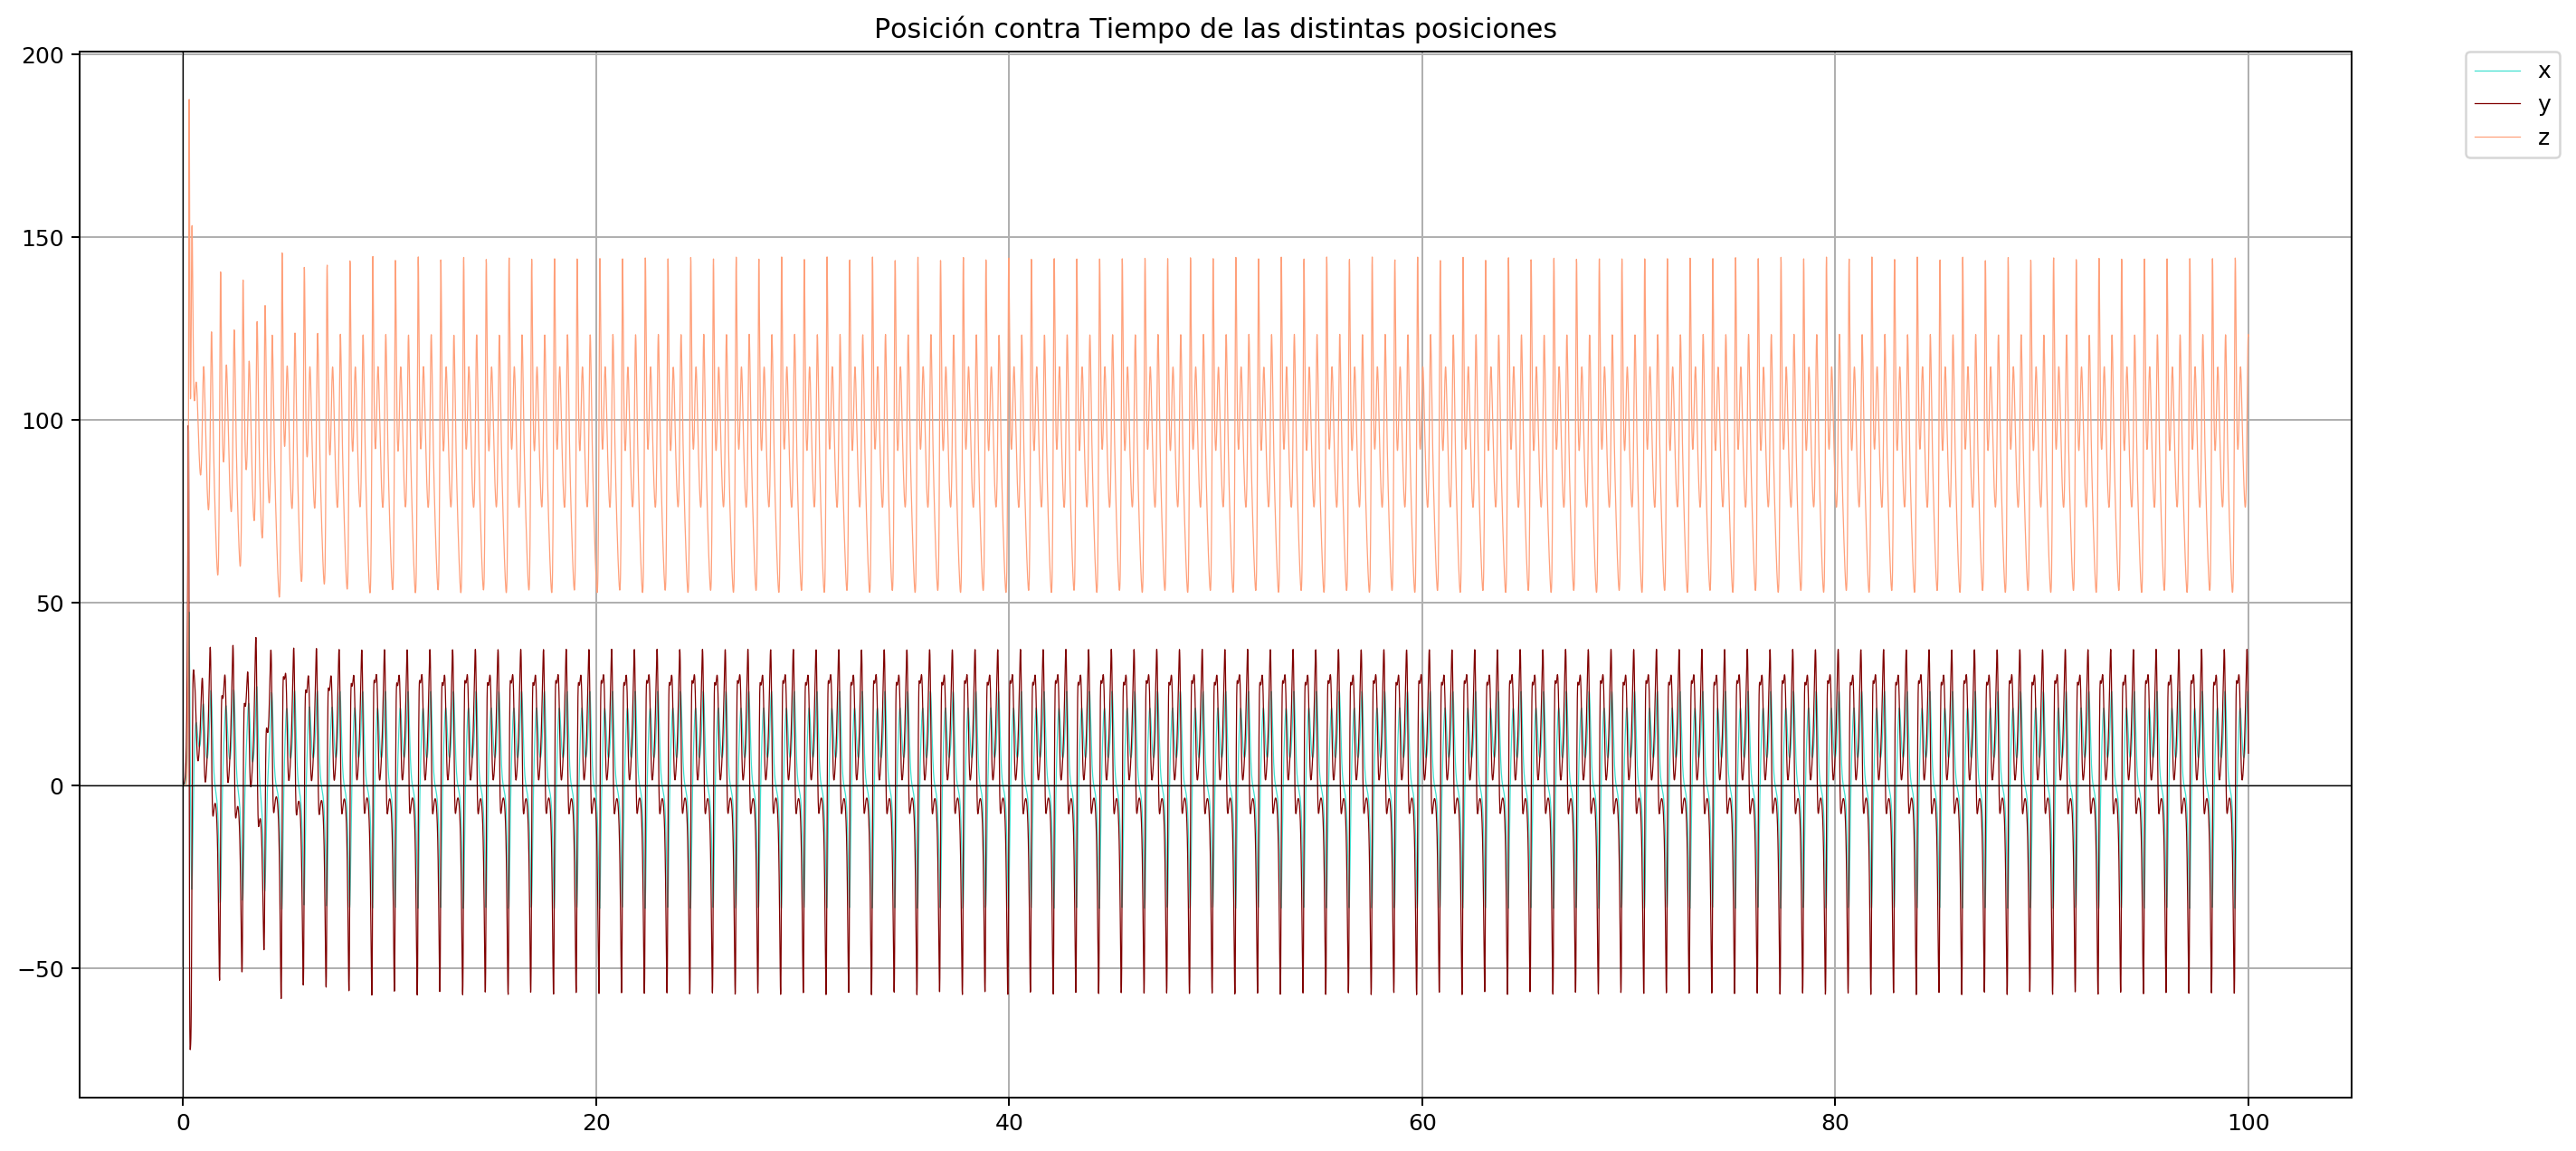
\includegraphics[width=5in]{AtractorLorentzPosicion3.png}
\end{figure}

El sistema se mueve mucho mas rápido y de una forma mas caótica que en casos anteriores, reforzando que si se mueve un solo parámetro, el sistema cambia totalmente. Algo que si tiene de parecido con los ejemplos anteriores, es que z siempre toma valores positivos, mientras que x y $y$ toman tanto positivos como negativos.

\section{Conclusiones}
Al terminar esta evaluación me di cuenta que el el utilizar herramientas como Python nos permite observar con mayor facilidad distintos sistemas y como es su funcionamiento. No solamente para su solución analítica, sino también para su interpretación mediante el uso de gráficas tanto en 3D como 2D. \\

A pesar de los distintos contratiempos dados en la evaluación, se pudo realizar todas las graficas, además de la animación o "gif" del retrato de fase. Esta evaluación se me hizo muy interesante, tanto la forma que se usa este lenguaje de programación, como el tema del que trato. Ver la animación del retrato de fase en 3D permite ver con mayor facilidad como evoluciona la posición con la velocidad y las planos coordenados complementan muy bien la información.

\section{Bibliografía empleada}
\begin{itemize}
    \item Lorenz System. (26 de Abril de 2018). Recuperado de: en.wikipedia.org/wiki/Lorenz\_system
    \item Animating the Lorenz Attractor with Python. (30 de Diciembre de 2016). Consultado el 26 de Abril de 2018. Recuperado de: geoffboeing.com/2016/12/animating-lorenz-attractor-python/
    
    \item Visual Analysis of Nonlinear Dynamical Systems. (2016).  Consultado el 26 de Abril de 2018. Recuperado de: www.mdpi.com/2079-8954/4/4/37/htm\#sec4-systems-04-00037
\end{itemize}

\end{document}